\section{Related Work}
\label{sec:related-work}

\begin{figure}[t]
	\centering
	\vspace*{-0.3cm}
	\hspace*{-0.4cm}
	\begin{minipage}[t]{0.3\textwidth}
		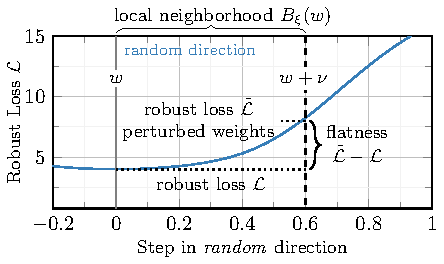
\includegraphics[width=0.9\textwidth]{fig_main_illustration3}
	\end{minipage}
	\begin{minipage}[t]{0.12\textwidth}
		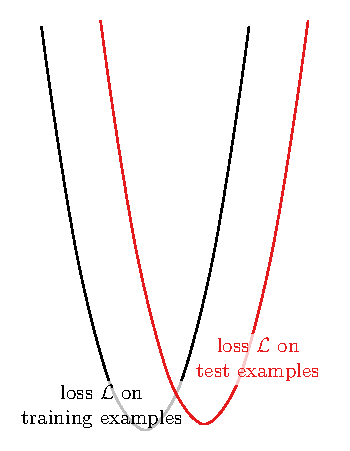
\includegraphics[width=1.2\textwidth]{fig_main_illustration2} 
	\end{minipage}
	\vspace*{-10px}
	\caption{\textbf{Measuring Flatness.} \textbf{Left:} Illustration of measuring flatness in a random (\ie, average-case, {\color{colorbrewer2}blue}) direction by computing the difference between \RCE $\tilde{\mathcal{L}}$ \emph{after} perturbing weights (\ie, $w + \nu$) and the ``reference'' \RCE $\mathcal{L}$ given a local neighborhood $B_\xi(w)$ around the found weights $w$, see \secref{subsec:main-flatness}. In practice, we average across/take the worst of several random/adversarial directions.
	\textbf{Right:} Large changes in \RCE around the ``sharp'' minimum causes poor generalization from training ({\color{colorbrewer0}black}) to test examples ({\color{colorbrewer1}red}).
	}
	\label{fig:main-illustration}
	\vspace*{-6px}
\end{figure}

\textbf{Adversarial Training (AT):}
Despite a vast amount of work on adversarial robustness, \eg, see \cite{SilvaARXIV2020,YuanARXIV2017,AkhtarACCESS2018,BiggioCCS2018,XuARXIV2019}, adversarial training (AT) has become the de-facto standard for (empirical) robustness. Originally proposed in different variants in \cite{SzegedyICLR2014,MiyatoICLR2016,HuangARXIV2015}, it received considerable attention in \cite{MadryICLR2018,robustness} and has been extended in various ways:
\cite{LambAISEC2019,CarmonNIPS2019,UesatoNIPS2019} utilize interpolated or unlabeled examples, \cite{TramerNIPS2019,MainiICML2020} achieve robustness against multiple threat models, \cite{StutzICML2020,LaidlawARXIV2019,WuICML2018} augment AT with a reject option, \cite{YeNIPS2018,LiuICLR2019b} use Bayesian networks, \cite{TramerICLR2018,GrefenstetteARXIV2018} build ensembles, \cite{BalajiARXIV2019,DingICLR2020} adapt the threat model for each example, \cite{Wong2020ICLR,AndriushchenkoNIPS2020,VivekCVPR2020} perform AT with single-step attacks, \cite{HendrycksNIPS2019} uses self-supervision and \cite{PangNIPS2020} additionally regularizes features  -- to name a few directions. However, AT is slow \cite{ZhangNIPS2020} and suffers from increased sample complexity \cite{SchmidtNIPS2018} as well as reduced (clean) accuracy \cite{TsiprasICLR2019,StutzCVPR2019,ZhangICML2019,RaghunathanARXIV2019}. Furthermore, progress is slowing down. In fact, ``standard'' AT is shown to perform surprisingly well on recent benchmarks \cite{CroceICML2020,CroceARXIV2020b} when tuning hyper-parameters properly \cite{PangARXIV2020b,GowalARXIV2020}. In our experiments, we consider several popular variants \cite{WuNIPS2020,WangICLR2020,ZhangICML2019,CarmonNIPS2019,HendrycksNIPS2019}.

\textbf{Robust Overfitting:} Recently, \cite{RiceICML2020} identified \emph{robust} overfitting as a crucial problem in AT and proposed early stopping as an effective mitigation strategy. This motivated work \cite{SinglaARXIV2021,WuNIPS2020} trying to mitigate robust overfitting. While \cite{SinglaARXIV2021} studies the use of different activation functions, \cite{WuNIPS2020} proposes AT with \emph{adversarial weight perturbations} (AT-AWP) explicitly aimed at finding flatter minima in order to reduce overfitting. While the results are promising, early stopping is still necessary. Furthermore, flatness is merely assessed visually, leaving open whether AT-AWP \emph{actually} improves flatness in adversarial weight directions. We consider both average- and worst-case flatness, \ie, random and adversarial weight perturbations, to answer this question.

\textbf{Flat Minima} in the loss landscape, \wrt changes in the weights, are generally assumed to improve \emph{standard} generalization \cite{HochreiterNC1997}. \cite{LiNIPS2018} shows that residual connections in ResNets \cite{HeCVPR2016} or weight decay lead to \emph{visually} flatter minima. \cite{NeyshaburNIPS2017,KeskarICLR2017} formalize this concept of flatness in terms of \emph{average-case} and \emph{worst-case} flatness. \cite{KeskarICLR2017,JiangICLR2020} show that worst-case flatness correlates well with better generalization, \eg, for small batch sizes, while \cite{NeyshaburNIPS2017} argues that generalization can be explained using both an average-case flatness measure and an appropriate capacity measure. Similarly, batch normalization is argued to improve generalization by allowing to find flatter minima \cite{SanturkarNIPS2018,BjorckNIPS1018}. These insights have been used to explicitly regularize flatness \cite{ZhengARXIV2020c}, improve semi-supervised learning \cite{CicekICCVWOR2019} and develop novel optimization algorithms such as Entropy-SGD \cite{ChaudhariICLR2017}, local SGD \cite{TinICLR2020} or weight averaging \cite{IzmailovUAI2018}.
\cite{DinhICML2017}, in contrast, criticizes some of these flatness measures as not being scale-invariant.
We transfer the intuition of flatness to the \emph{robust} loss landscape, showing that flatness is desirable for adversarial robustness, while using scale-invariant measures.